\documentclass{article}

\usepackage{amsmath}

\usepackage{mathptmx}           
\usepackage{graphicx}           
\usepackage{url}            
\usepackage{subcaption}    


\usepackage[a4paper,margin=2cm]{geometry}

\usepackage{natbib} 
\usepackage[numbered, framed]{mcode}

\usepackage{lipsum}

%\usepackage{epstopdf}
%\epstopdfsetup{outdir=./}

\begin{document}

\author{H. Blum, D. Cavezza, A. Paudice and M. Rohbeck\\
 Machine Learning CO395\\
  Imperial College London}
\date{\today}
\title{Assignment 3: Neural Networks}
\maketitle

\section{Implementation}
In our second assignment, we apply neural networks to the emotion recognition problem. We use the Neural Network Toolbox provided by MATLAB to train and compare the performance of different neural networks on the dataset at our disposal, in order to find the best training algorithm along with the best parameter configuration.\\
We compare four different training algorithm:
\begin{itemize}
	\item Standard gradient descent backpropagation (\verb$traingd$ in MATLAB);
	\item Gradient descent with adaptive learning rate (\verb$traingda$);
	\item Gradient descent with momentum (\verb$traingdm$)
	\item Resilient backpropagation (\verb$trainrp$).
\end{itemize}
In this section we describe our implementation of:
\begin{itemize}
	\item selection of the best set of parameters for each algorithm;
	\item evaluation of NN's performance on unseen data.
\end{itemize}

\subsection{Parameter selection}
In the first part, we use cross- validation to select the best performing algorithm on the dataset and the best parameter configuration for it. Cross-validation is performed by splitting the dataset into 10 folds and using 9 folds for training and 1 for validation; iteratively, each fold is in turn used for validation, and ultimately the algorithm and parameter set that yield the best average performance over the folds is chosen.\\
For splitting, we use the same function as in the previous exercise, which performs \emph{stratified} cross-validation: each fold contains approximately the same proportion of examples in every class as the whole dataset. It is implemented in the file \verb$getFoldsPartitioning.m$.\\


\subsection{Performance evaluation}


\section{Performance results}


\section{Questions}
\subsection{Question 1}
We chose the optimal topology and parameters through cross-validation. In detail, in each iteration we tested the performance of the chosen topology on the fold used as validation set; at the end, we averaged the performances of each topology and parameters configuration and chose the setting that showed the best average performance.\\
We tested topologies with 1 and 2 layers. Topologies with 1 layer can fit any Boolean function, while 2-layer topologies can approximate arbitrarily well any real-valued function.\\
For each layer, a common practice is to use a number of neurons between the sizes of the input and the output layer. Choosing less neurons than the output leads to a data compression that may cause information loss before reaching the output.\\
For the algorithms' parameters, we had to trade off the number of tests executed and the total time for testing. We chose learning rates that covered different orders of magnitude where possible.\\
The optimal parameters for the standard gradient descent are:\\
Neurons per layer = 18; Number of layers = 2; Learning rate = 0.5; Avg Error = 0.0458\\
The optimal parameters for the adaptive gradient descent are:\\
Neurons per layer = 15; Number of layers = 2; Learning rate = 0.1; LR decrease rate = 0.7; LR increase rate = 1.4; Avg Error = 0.0449\\
The optimal parameters for the gradient descent with momentum are:\\
Neurons per layer = 42; Number of layers = 1; Learning rate = 1; Momentum coefficient = 0.9; Avg Error = 0.0679\\
The optimal parameters for resilient backpropagation are:\\
Neurons per layer = 14; Number of layers = 2; Delta increase = 1.3; Delta decrease = 0.5; Avg Error = 0.0444\\

%\section{Training}
%Decision trees are a conceptually simple, yet powerful model for solving classification problems. The ID3 algorithm is one of the simplest training algorithms for decision trees: it builds the tree by choosing at each step the attribute that maximizes the \emph{Information Gain}, a measure that represents the discriminatory power of an attribute over the class values.
%
%The problem we are given consists in classifying facial expressions into 6 emotion classes via decision trees; each facial expression is represented as a feature vector of 45 \emph{Action Units} (AU), where each feature is a binary value that indicates the presence or absence of each AU in the example. We decompose the problem in 6 binary decision problems according to the \emph{1-vs-all model}, with each problem corresponding to the recognition of one specific emotion. Therefore, we use ID3 to train 6 different trees, each one trained to recognize one specific emotion.
%
%Our implementation of the ID3 algorithm is provided in the files \verb$train.m$, \verb$DTTrain.m$ and \verb$choose_best_attr.m$, containing the functions with the same name.
%
%The function \verb$train$ is the entry point for the training algorithm. It takes as inputs the training examples, the array of attribute ids (in our case, an array from 1 to 45), and an array of labels of the same length as the number of examples; such labels are numbers from 1 to 6, each one indicating one of the emotions in the original dataset. It returns the 6 desired trees.
%
%Each tree is trained on a transformed version of the input data: at the i-th iteration of the for loop, the labels are made binary; the vector \verb$binary_targets$ contains a 1 in the positions corresponding to the i-th emotion, a 0 in all the other positions. The function \verb$DTTrain$ is called to train each tree on such transformed data.
%
%\begin{lstlisting}
%function [ T ] = train( examples, attributes, labels )
%%Train 6 binary trees on the training set (examples, labels) and return
%%them into the tree array T.
%
%[m, n] = size(examples); 
%binary_targets = zeros(m, 1);
%
%for i = 1:6
   %
    %%Switch to binary labels
    %index = find(labels == i);
    %binary_targets(index) = 1;
    %
    %%Train a tree to learn an emotion
    %T(i) = DTTrain(examples, attributes, binary_targets);
    %
%%    DrawDecisionTree(T(i));
    %
    %binary_targets = zeros(m, 1);
    %
%end
%
%end
%\end{lstlisting}
%The function \verb$DTTrain$ is a recursive function implementing the ID3 algorithm. Every time a recursion occurs, a check is performed on the entropy of the current node: if it is not 0, the attribute that maximizes the Information Gain is chosen and associated to the current node, then the recursion occurs.\\
%In the first call the function is passed the whole training sample, the array 1:45 of attribute ids, and the binary labels.
%\begin{lstlisting}
%function [ tree ] = DTTrain( examples, attributes, binary_targets )
%%Train a decision tree on the dataset (examples, binary_target)
%%according to the ID3 algorithm. The examples have the attributes listed in
%%attributes
%\end{lstlisting}
%First an empty tree is initialized.
%\begin{lstlisting}[firstnumber=6]
%%Initialize an empty tree
%tree.op = [];
%
%tree.kids = [];
%tree.class = [];
%\end{lstlisting}
%Then a check on the input's entropy is performed. If the sample entropy in the labels is 0, the algorithm is in a pure node, that is all the current examples belong to the same class: in such case, the algorithm must stop, and the value returned by the current node is the class value held by the majority of the examples. Likewise, the algorithm must stop if there are no more attributes to decide about. In these cases, \verb$tree.op$ and \verb$tree.kids$ are not set, so as to mark the node as a leaf.
%\begin{lstlisting}[firstnumber=12]
%if (sample_entropy(binary_targets) == 0 || isempty(attributes))   
    %% either pure targets or no more attributes to base decision on
    %
    %tree.class = maj_value(binary_targets);
%\end{lstlisting}
%Else, the attribute that yields the highest Information Gain is chosen
%\begin{lstlisting}[firstnumber=17]
%else
    %
    %tree.op = choose_best_attr(examples, attributes, binary_targets);
%\end{lstlisting}
%and the examples are split by the value they contain in the chosen attribute.
%\begin{lstlisting}
    %tree.kids = cell(1, 2);
        %
    %% raise up the kids
    %
    %for j = 1:2
        %
        %%fprintf('#Examples: %d \n', length(examples));
        %child_index = find(examples(:, tree.op) == (j - 1));
        %child_examples = examples(child_index, :);     
        %child_binary_targets = binary_targets(child_index);
%\end{lstlisting}
%At this point, the set of examples with a specific value of the chosen attribute may be empty. In that case, the corresponding kid node is made leaf and the returned class value is the value held by the majority of the nodes in the current node.
%\begin{lstlisting}[firstnumber=36]
        %if (isempty(child_examples))
            %% we can't train this child, make a leaf with the majority
            %% value of all training data coming to the parent
            %
            %tree.kids{j}.op = [];
            %tree.kids{j}.kids = [];
            %tree.kids{j}.class = maj_value(binary_targets);
%\end{lstlisting}
%Otherwise, the corresponding subtree is created. Note that in the recursive calls, the chosen attribute is deleted from the list of candidate attributes, since its value is fixed for the samples in each of the kids (0 for the left kid and 1 for the right).
%\begin{lstlisting}[firstnumber=44]
        %else 
            %
            %% remove the used attribute from the list
            %index = find(attributes == tree.op);
            %attributes(index) = [];
            %
            %% recursive training with this child
            %tree.kids{j} = DTTrain(child_examples, attributes, ...
                %child_binary_targets);
                    %
        %end
%\end{lstlisting}
%At line 19, the above function calls \verb$choose_best_attr$. This function computes the Information Gain of every available attribute and returns the id of the attribute that yields the highest Information Gain.
%\begin{lstlisting}
%function [ best_attr ] = choose_best_attr( examples, attributes, binary_targets )
%%chooseBestAtt computes and return in bestAtt the attribute in attributes
%%which determine the maximum information gain for the set 
%%(examples, binary_targets). Return -1 if the set is pure because no split
%%is required
%
%%Compute the sample entropy
%n_ex = length(binary_targets);         %Dataset size
%E = sample_entropy(binary_targets); %Sample entropy
%
%% initial values
%best_gain = 0;
%best_attr = attributes(1); % for now this is as good as anything
    %
%for i = 1:length(attributes)
       %
    %% examples where attribute is 1
    %one_attr = binary_targets(examples(:, attributes(i)) == 1); 
    %% examples where attribute is 0
    %zero_attr = binary_targets(examples(:, attributes(i)) == 0);
        %
    %E_partition = length(one_attr)/n_ex * sample_entropy(one_attr) ...
        %+ length(zero_attr)/n_ex * sample_entropy(zero_attr);
        %
    %gain = E - E_partition;
        %
    %if (gain > best_gain)
            %
       %best_gain = gain;
       %best_attr = attributes(i);
        %
    %end
        %
%end
%
%end
%
%\end{lstlisting}
%Finally, the files \verb$sample_entropy.m$ and \verb$maj_value.m$ simply contain the computation of the entropy and the most frequent label value in a sample respectively.\\
%The learned trees are shown in Figures~\ref{fig:trees}-\ref{fig:noisytrees}.
%\begin{figure}
 %\centering
 %\begin{subfigure}[b]{.49\textwidth}
   %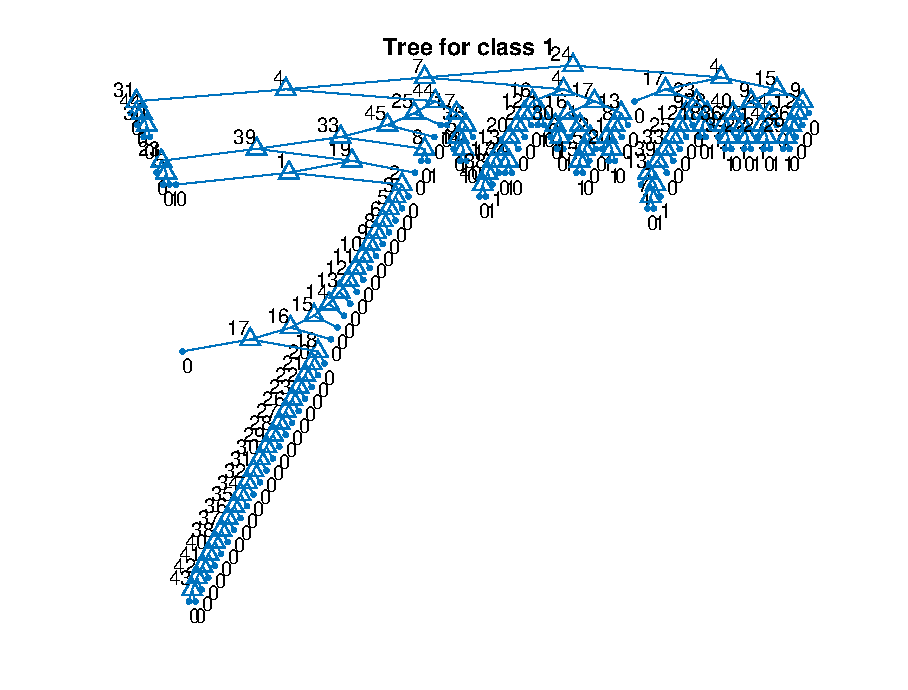
\includegraphics[width=\textwidth]{tree1.eps}
 %\end{subfigure}
 %\begin{subfigure}[b]{.49\textwidth}
   %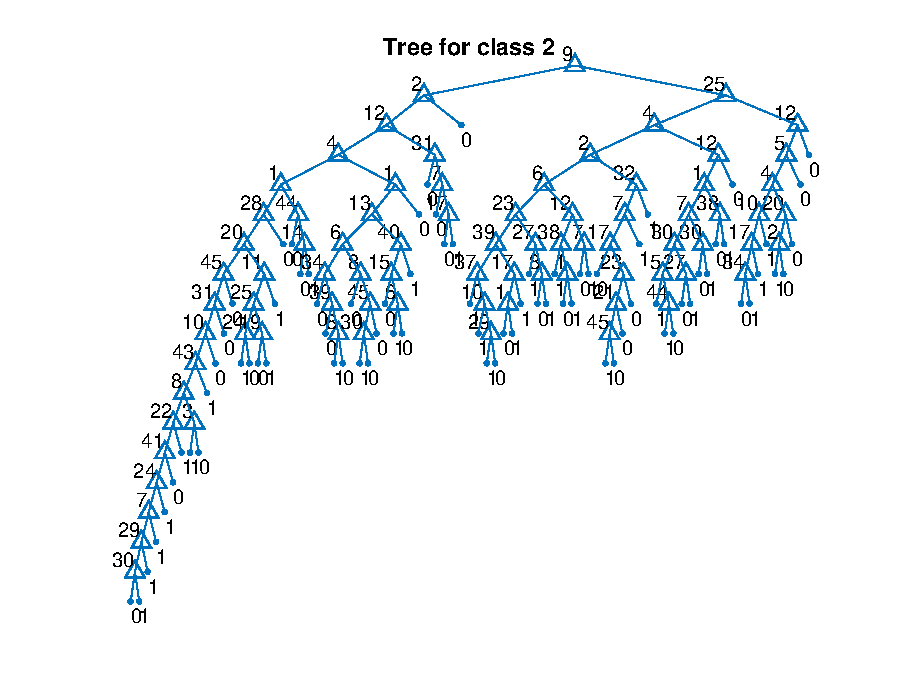
\includegraphics[width=\textwidth]{tree2.eps}
 %\end{subfigure}
 %\begin{subfigure}[b]{.49\textwidth}
   %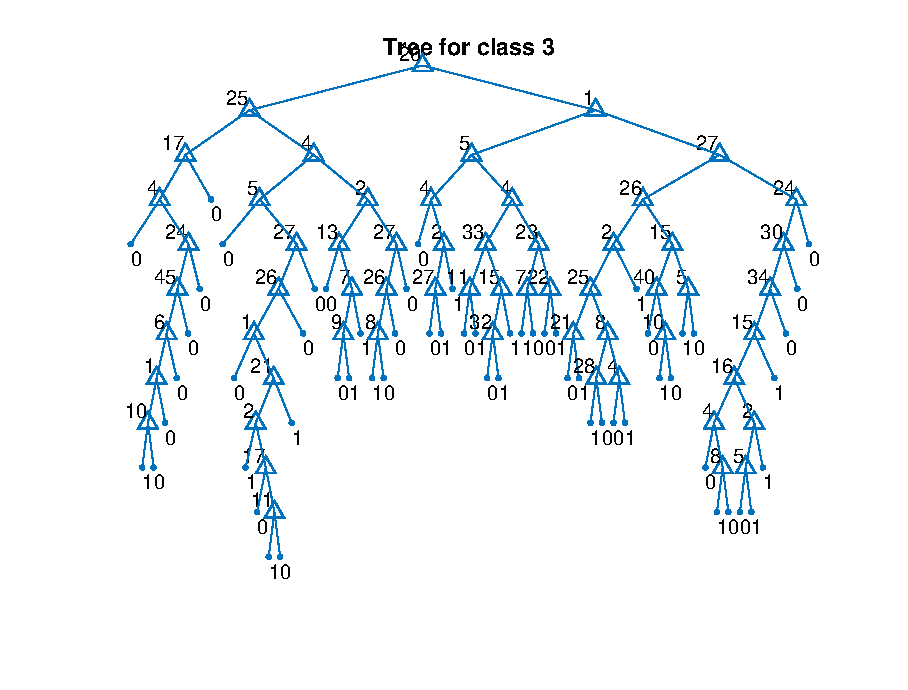
\includegraphics[width=\textwidth]{tree3.eps}
 %\end{subfigure}
 %\begin{subfigure}[b]{.49\textwidth}
   %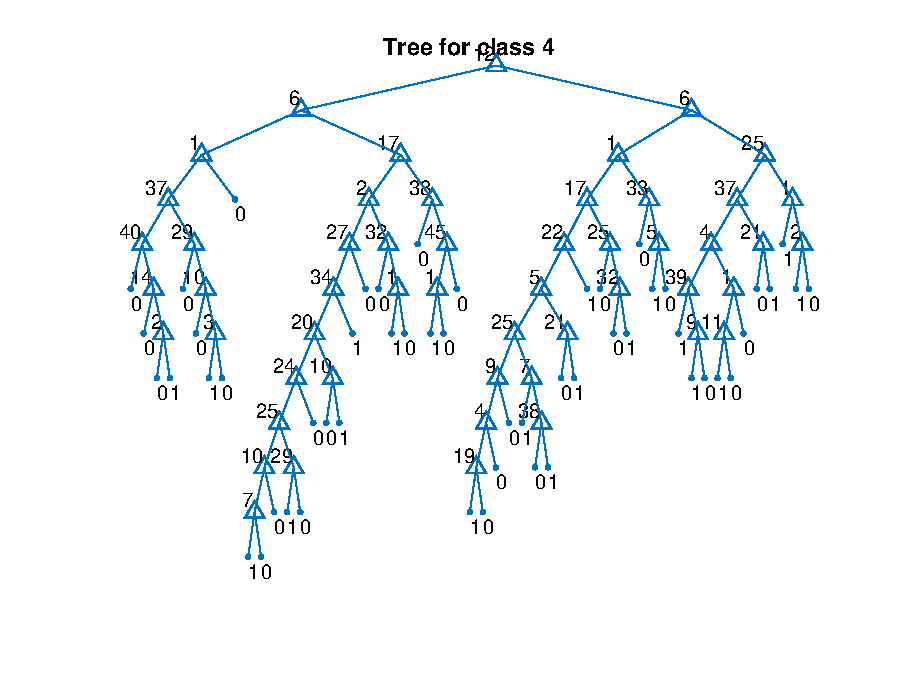
\includegraphics[width=\textwidth]{tree4.eps}
 %\end{subfigure}
 %\begin{subfigure}[b]{.49\textwidth}
   %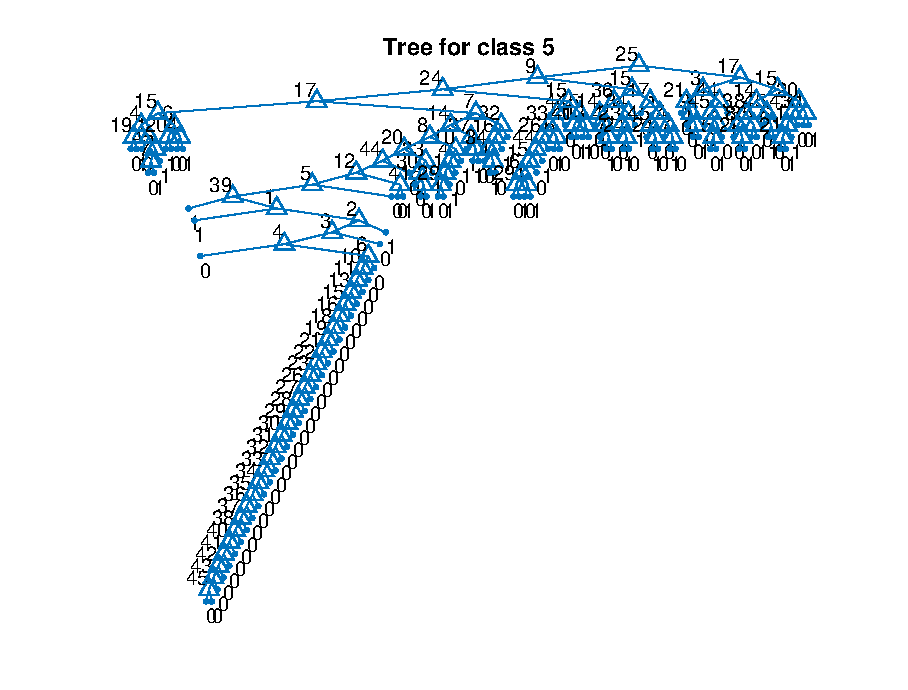
\includegraphics[width=\textwidth]{tree5.eps}
 %\end{subfigure}
 %\begin{subfigure}[b]{.49\textwidth}
   %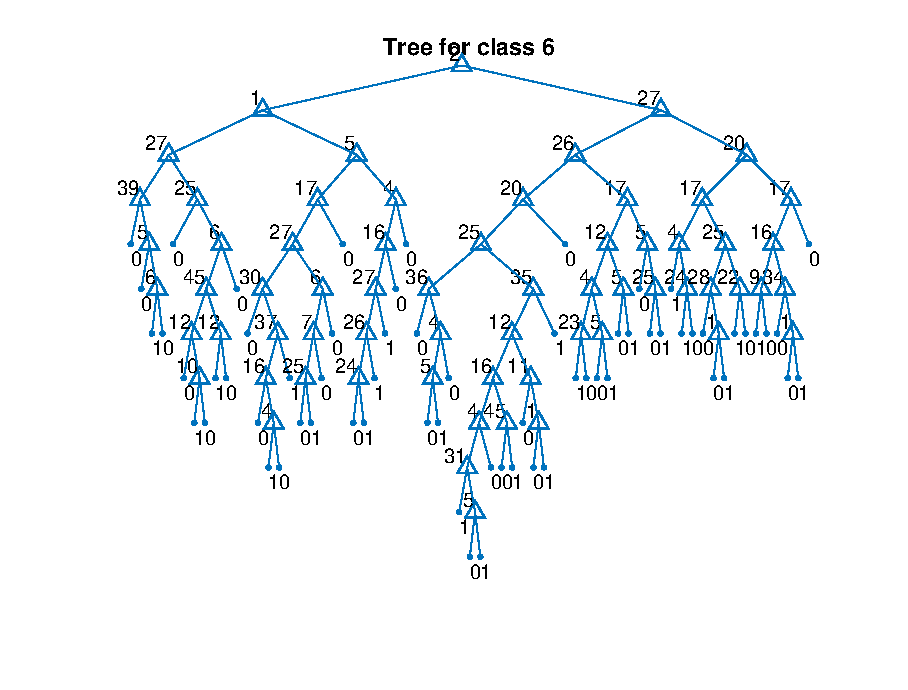
\includegraphics[width=\textwidth]{tree6.eps}
 %\end{subfigure}
 %\caption{Trees learnt on clean data}
 %\label{fig:trees}
%\end{figure}
%\begin{figure}
 %\centering
 %\begin{subfigure}[b]{.49\textwidth}
   %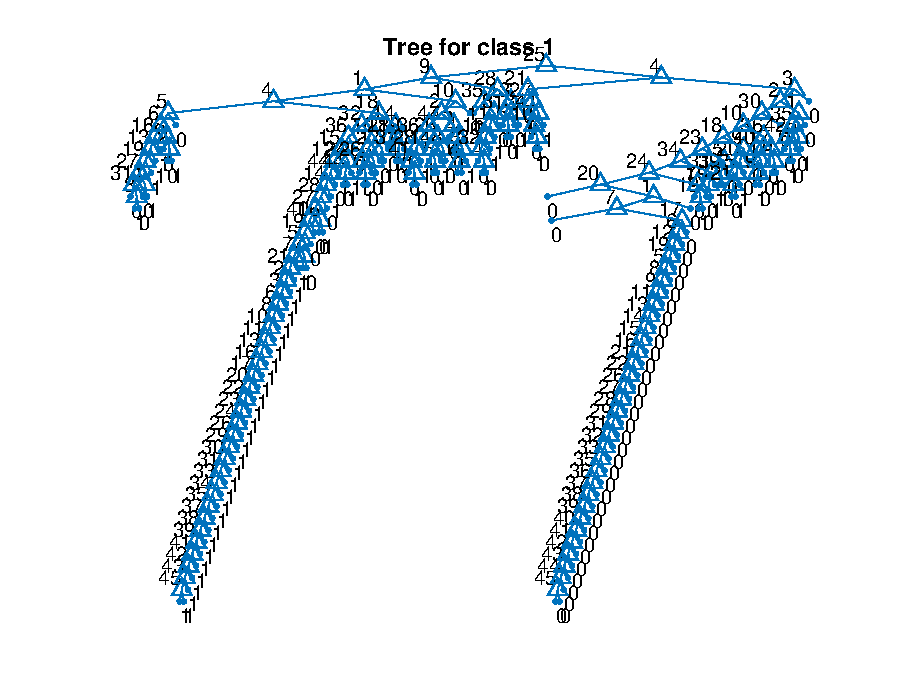
\includegraphics[width=\textwidth]{noisytree1.eps}
 %\end{subfigure}
 %\begin{subfigure}[b]{.49\textwidth}
   %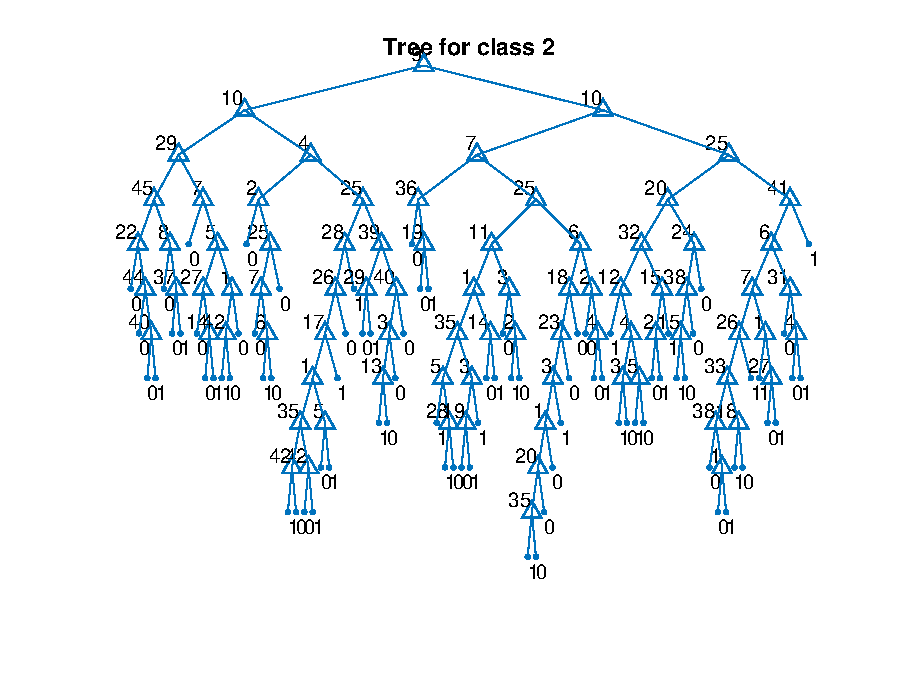
\includegraphics[width=\textwidth]{noisytree2.eps}
 %\end{subfigure}
 %\begin{subfigure}[b]{.49\textwidth}
   %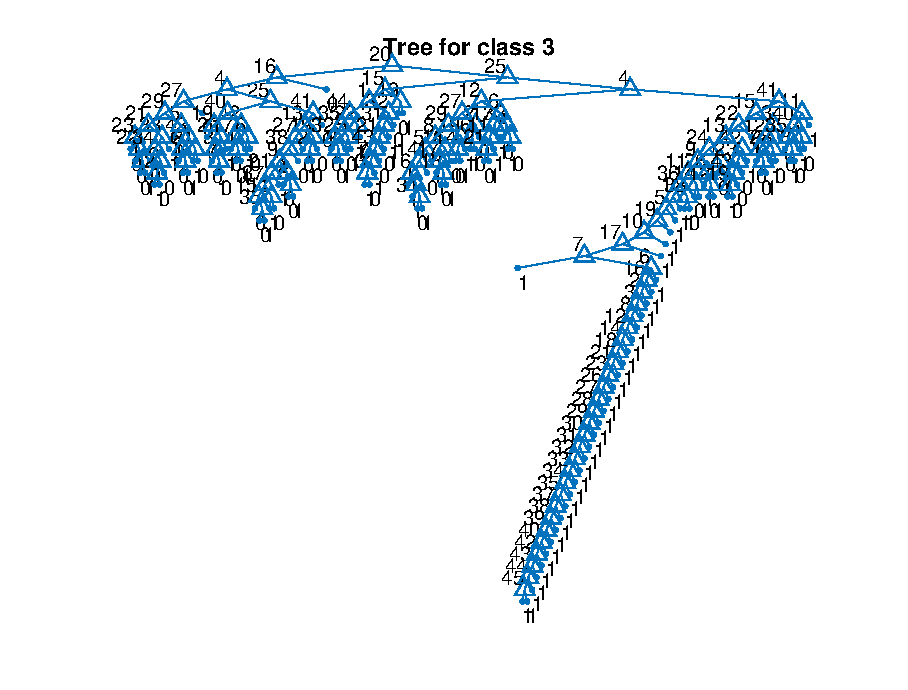
\includegraphics[width=\textwidth]{noisytree3.eps}
 %\end{subfigure}
 %\begin{subfigure}[b]{.49\textwidth}
   %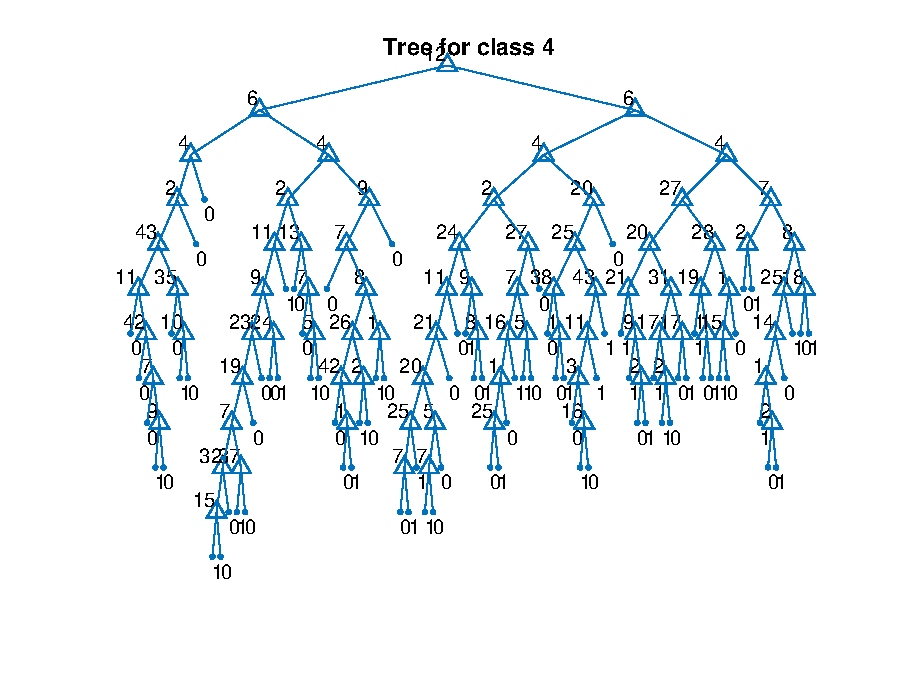
\includegraphics[width=\textwidth]{noisytree4.eps}
 %\end{subfigure}
 %\begin{subfigure}[b]{.49\textwidth}
   %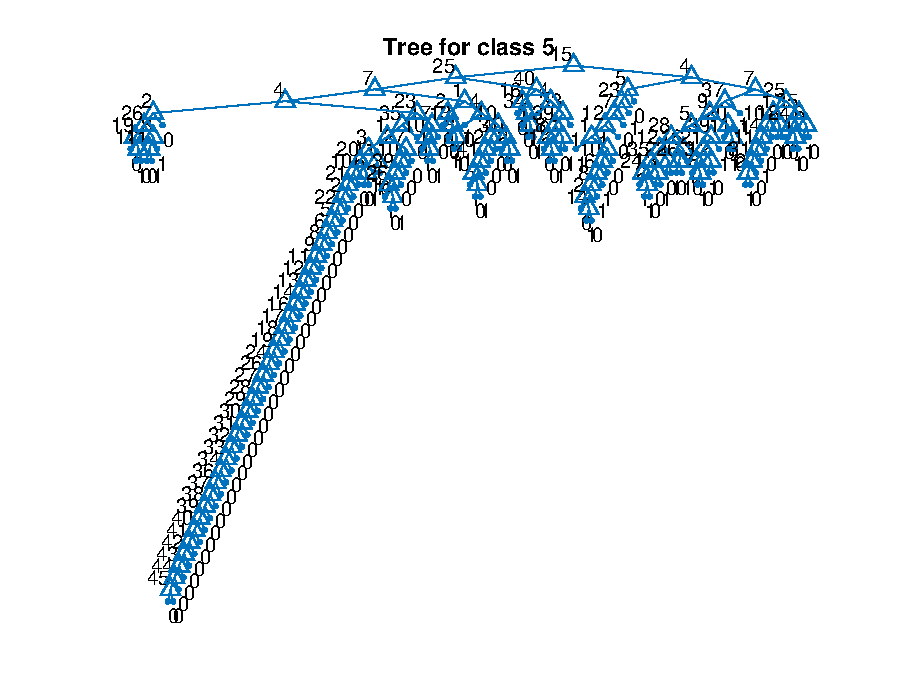
\includegraphics[width=\textwidth]{noisytree5.eps}
 %\end{subfigure}
 %\begin{subfigure}[b]{.49\textwidth}
   %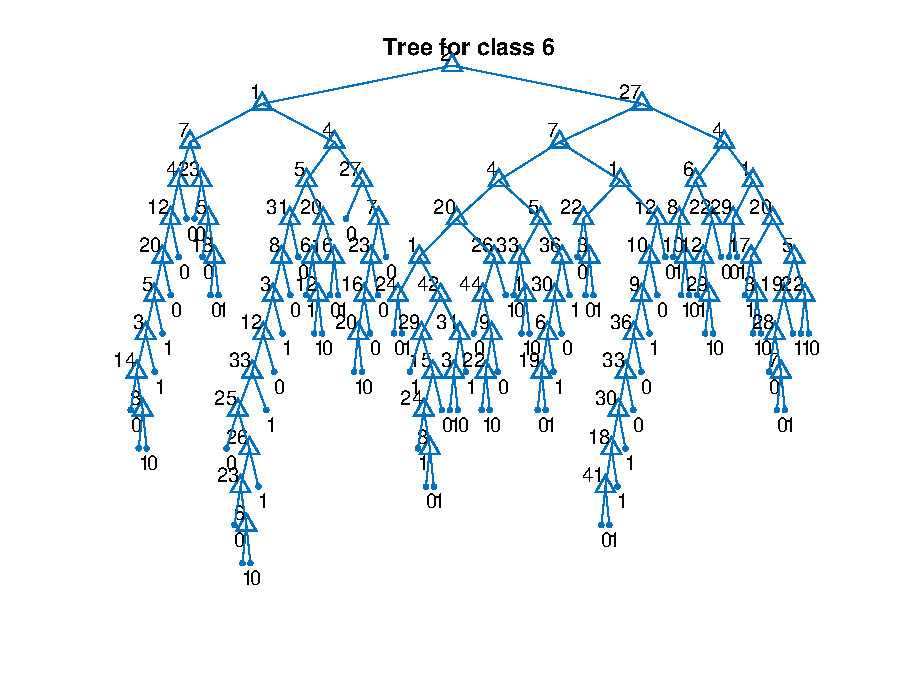
\includegraphics[width=\textwidth]{noisytree6.eps}
 %\end{subfigure}
 %\caption{Trees learnt on noisy data}
 %\label{fig:noisytrees}
%\end{figure}
%
%
%\newpage
%
%\section{Decision making strategies}
%\label{sec:decision_strategies}
%Since we have different trees, and each of these trees may commit mistakes in its classification, their outputs may be contradictory. Specifically, more than one tree may return 1 in response to the same example, or all trees may return 0. Therefore, we have devised different decision policies to resolve conflicts.
%
%\subsection{Random choice}
%One possible strategy is choosing randomly: if more than a tree returns 1, the label of the example is chosen randomly among the classes corresponding to such trees; if all the trees return 0, the label is picked randomly among all the classes.\\
%The implementation of this strategy is in the file \verb$testTreesRandomChoice.m$.
%\begin{lstlisting}
%function [ predictions ] = testTreesRandomChoice(T,x2)
%% TestTreesRandomChoice performs a random selection among the emotions of
%% all the trees that return a prediction of 1, or among all the emotions if
%% all the trees return 0.
%
%[m,n] = size(x2);
%binary_predictions = zeros(m,6);
%predictions = zeros(m,1);
%
%for i = 1:m
    %for j = 1:6
        %binary_predictions(i,j) = predictionBinaryTree(T(j),x2(i,:));
    %end
    %% If all the predictions are 0, pick an emotion randomly
    %if(max(binary_predictions(i,:))==0)
        %predictions(i) = randi(6);
    %% Else pick an emotion randomly among the 1s
    %else
        %candidateEmotions = find(binary_predictions(i,:));
        %predictions(i) = candidateEmotions(randi(length(candidateEmotions)));
    %end
    %
%end
%
%
%end
%\end{lstlisting}
%The function \verb$predictionBinaryTree$ called in line 12 is defined in the same file: it passes through the branches of the tree corresponding to the attribute values of the input example and returns the binary label corresponding to the reached leaf.
%\begin{lstlisting}[firstnumber=28]
%function [ class ] = predictionBinaryTree( tree, x )
%%predictionBinaryTree walks along the tree to find the classification of
%%the istance x
    %
    %if (isempty(tree.op))   %Check if it is a leaf
        %
        %class = tree.class;
        %
    %else                    %Test the attribute
        %
        %x_to_test = x(tree.op);
        %
        %if (x_to_test == 0) %Follow the left branch
           %
           %class = predictionBinaryTree(tree.kids{1}, x);
            %
        %else %Follow the right branch
            %
           %class = predictionBinaryTree(tree.kids{2}, x);
            %
        %end
        %
    %end
%
%end
%\end{lstlisting}
%This strategy is one of the simplest to consider in resolving conflicts. It is chosen as our baseline strategy.
%
%\subsection{Score-based choice}
%Our second strategy is about choosing the label with the highest score. In this implementation, we assign a score to each leaf of every tree between 0 and 1. The score is correlated to the number of training examples that can be classified by the given leaf with respect to the total number of training examples in every class.
%\begin{align*}
    %\textrm{score} = \frac{\textrm{\# correctly classified training data by this leaf}}{\textrm{\# training data in this tree}}
%\end{align*}
%Of all binary classification trees returning 1, the decision algorithm will pick the class corresponding to the tree with the highest decision score. If no tree returns 1, it will pick at random.
%\begin{lstlisting}
%function [ predictions ] = decide_by_score(trees, testset)
%% decide_by_score performs a classification based on the fraction of
%% correctly classified training examples given by the tree leafs
%
%[m,n] = size(testset);
%predictions = zeros(m,1);
%
%for i = 1:m
    %% test in all trees, find the one with the best score
    %best_score = 0;
    %predictions(i) = NaN;
    %for t = 1:6
        %[pred, score] = prediction_with_score(trees(t),testset(i,:));
        %if pred == 1
            %% the tree recognises this item as his class
            %if score > best_score
                %predictions(i) = t;
                %best_score = score;
            %end
        %end
    %end
    %% If all the predictions are 0, pick a random class
    %if(isnan(predictions(i)))
        %predictions(i) = randi(6);
    %end
%end
%
%end
%\end{lstlisting}
%
%\subsection{Tree confidence choice}
%With this decision strategy, in case of a tie, we choose the tree which achieved the smallest classification error on the training set. The key assumption here is that a tree with a small classification error represents a confident model, while a tree with a high classification error is less confident. This assumption is justified observing that a tree with small confidence is likely to be a poor model of the true function because of underfitting. 
%
%In particular, this function first computes the classification error achieved by every tree on the training set (lines 39-52). Then it computes the predictions made by the trees for each point in the test set (lines 57-65). Finally, it checks whether there is a tie between two or more trees and makes the final prediction picking the tree with the smallest training classification error (lines 68-84). The implementation of this strategy is in the file \verb$testTreesTreeConfidence.m$.
%
%\begin{lstlisting}[firstnumber=28]
%function [ predictions ] = testTreesTreeConfidence( T, x, y, test_data )
%
%[m, n] = size(test_data);
%binary_predictions = zeros(m, 6);
%binary_errors = zeros(1, 6);
%confidence = zeros(1, 6);
%predictions = zeros(m, 1);
%
%[m_train, n_train] = size(x);
%
%%Evaluate the error in the training set
%for i = 1:6
%
    %for j = 1:m_train
        %
        %binary_predictions(j, i) = predictionBinaryTree(T(i), x(j, :));
        %binary_errors(i) = binary_errors(i) + (not(binary_predictions(j, i)==1 && y(j)==i)...
            %&& not(binary_predictions(j, i)==0 && y(j)~=i));
   %
    %end
    %
    %binary_errors(i) = 1/m_train * binary_errors(i);
    %confidence(i) = 1 - binary_errors(i);
%
%end
%
%binary_predictions = zeros(m, 6);
%
%%Compute the predictions of each tree
%for i = 1:6
%
    %for j = 1:m
        %
        %binary_predictions(j, i) = predictionBinaryTree(T(i), test_data(j, :));
   %
    %end
%
%end
%
%%Compute the prediction
%for i = 1:m
    %candidateClasses = find(binary_predictions(i,:)==1);
    %if(isempty(candidateClasses))
        %% If all the trees return 0, pick the prediction with minimum
        %% confidence. This prediction, indeed, is the most error-prone and
        %% most likely its correct value should be 1 (only according to our
        %% confidence heuristic, there is no mathematical justification
        %% here)
        %[~, predictions(i)] = min(confidence);
    %else
        %% Take the prediction of the tree with most confidence among the
        %% ones returning 1
        %[~, imaxConfidence] = max(confidence(candidateClasses));
        %predictions(i) = candidateClasses(imaxConfidence);
    %end
%
%end
%
%end
%
%function [ class ] = predictionBinaryTree( tree, x )
%%predictionBinaryTree walks along the tree to find the classification of
%%the istance x
    %
    %if (isempty(tree.op))   %Check if is a leaf
        %
        %class = tree.class;
        %
    %else                    %Test the attribute
        %
        %x_to_test = x(tree.op);
        %
        %if (x_to_test == 0) %Follow the left branch
           %
           %class = predictionBinaryTree(tree.kids{1}, x);
            %
        %else %Follow the right branch
            %
           %class = predictionBinaryTree(tree.kids{2}, x);
            %
        %end
        %
    %end
%
%end
%\end{lstlisting}
%
%This function makes use of \verb$predictionBinaryTree$, defined above. 
%
%\subsection{Simplest Hypothesis}
%Our last strategy was choosing the label which was found by going the lowest number of nodes down the tree. This approach should effectuate that less wrong decisions are made because a decision based on less attributes should be less prone to overfitting.
%\begin{lstlisting}
%function [ predictions ] = testTreesSimplestHypothesis( T, test_data )
%%testTreesSimplestHypothesis makes prediction on the unseen data test_data using the 6 trees
%%in T and returns the results in predictions. The decision method chooses
%%the label which is found by the node with the lowest depth in case of a tie.
%
%[m, ~] = size(test_data);
%binary_predictions = zeros(m, 6);
%depth_predictions = zeros(m, 6);
%predictions=zeros(m,1);
%
%for i = 1:m
    %
    %for j = 1:6
        %
        %c=1;                    % counter             
        %tree=T(j);              % testing Tree 
        %done=0;
        %class=-1; 
        %
        %while done ~=1          % count depth and find class
            %[tree,test_data(i,:), done, class] = predictionBinaryTree(tree,test_data(i,:));
            %c=c+1;
        %end
        %
        %binary_predictions(i, j) = class;           % save labels
        %depth_predictions(i, j) = c;                % save depth
        %
    %end
    %
%end
%
%for i=1:m
    %if sum(binary_predictions(i,:))>1                           % more than one label found
        %a=depth_predictions(i,:).*binary_predictions(i,:);  
        %a(a==0)=46;
        %[~,predictions(i)]=min(a);                              % choose minimum depth
    %elseif sum(binary_predictions(i,:))==1
        %[~, predictions(i)] = max(binary_predictions(i,:),[],2);    % only one label assigned
    %else                                                        % all labels are 0
        %predictions(i)=1;                                      
    %end
%end
%
%end
%\end{lstlisting}
%The second part is just a modified version of the \verb$predictionBinaryTree$ function from the random Choice with integrated counting of nodes.
%\begin{lstlisting}[firstnumber=45]
%function [tree, x, done, class ] = predictionBinaryTree( tree, x)
%%predictionBinaryTree walks along the tree to find the classification of
%%the istance x and calculates the depth
%done=0;
%class=-1;
%
%if (isempty(tree.op))   %Check if it is a leaf
    %
    %class = tree.class;
    %done = 1;           % counting done
    %
%else                    %Test the attribute
    %
    %x_to_test = x(tree.op);
    %
    %if (x_to_test == 0) %Follow the left branch
        %
        %tree = tree.kids{1};
        %
    %else %Follow the right branch
        %
        %tree = tree.kids{2};
        %
    %end   
%end
%end
%\end{lstlisting}
%
%\newpage
%\section{Cross-validation}
%\emph{Cross-validation} is generally used to obtain an appropriate estimate of the performance of a model on unseen data, or to tune the parameters of a model appropriately (i.e. to perform model selection), if the size of the data set at one's disposal is low.\\
%It consists in splitting the data set into k partitions, called \emph{folds}, and testing the training algorithm iteratively on these folds. In each iteration k-1 folds are used to train the model, while the remaining one is used for testing or validating the trained model. After k iterations, the performances computed in each fold are averaged.\\
%Such partitioning and iterations are necessary for two reasons:
%\begin{itemize}
	%\item the performance statistics computed on the same data used for training are not reliable estimates of the generalization power of the learnt model; thus, it is necessary to leave some data outside the training set for testing purposes;
	%\item the performance statistics are more reliable as the test set size increases; iterating over all the folds is a device to increase the number of examples on which the learnt model is tested.
%\end{itemize}
%We provide an implementation of \emph{stratified} cross-validation: in this version, the proportion of class values inside each fold reproduces approximately the proportion of class values inside the entire dataset. Our implementation is provided in the five m-files \verb$crossValidate.m$, \verb$stratifySampleIndexed.m$, \verb$getFoldIndexed.m$, \verb$getTrainingSetIndexed.m$, and \verb$getTestSetIndexed.m$.\\
%The function \verb$crossValidate$ requires as inputs the attributes and label values of every example, and the number of desired folds; \verb$stratified$ is a Boolean parameter specifying whether or not the cross-validation should be stratified.
%\begin{lstlisting}[breaklines=true]
%function [confusionMatrix, accuracy, precision, recall, fmeasure] = crossValidate(xvalues, labels, k, stratified)
%\end{lstlisting}
%If \verb$stratified$ is \verb$false$, the function just performs a split of the data set into k folds (lines 27-31). Otherwise, the split is performed according to the stratified cross-validation (lines 15-25). First, the dataset is split by class value (line 16); then, each fold is constructed by taking a subfold from the examples of each class, and concatenating such subfolds (lines 18-25).
%\begin{lstlisting}[firstnumber=14]
%if(stratified)
    %% Obtain the example indices divided by class label
    %indicesPerClass = stratifySampleIndexed(labels);
    %
    %for i=1:k
        %% Perform the division in k folds in every class. Merge the
        %% subfolds from all the classes to obtain a single fold
        %for j=1:numClasses
            %foldsIndices{i} = [foldsIndices{i}; getFoldIndexed(indicesPerClass{j},k,i)];
        %end
        %
    %end    
    %
%else
    %% Non-stratified cross-validation
    %for i=1:k
        %foldsIndices{i} = getFoldIndexed(1:length(labels),k,i);
    %end
%end
%\end{lstlisting}
%Notice that there is no randomness in the split: if the input is the same, the folds will not change over different calls.\\
%After the split, the training and test sets are constructed for each iteration, the performance indicators are computed for each fold and the averages are returned. For further details, refer to the indicated files and their comments.
%
%\newpage
%\section{Performance}
%We report the performance of a 10-fold stratified cross-validation executed on each of the decision strategies presented in Section~\ref{sec:decision_strategies}. Figures~\ref{fig:perfRandom}-\ref{fig:perfTreeConf} show the total confusion matrix (that is the sum of confusion matrices over all the folds) and the average performance metrics over the 10 folds.\\
%\begin{figure}
    %\hspace*{\fill}%
    %\subcaptionbox{Confusion matrix for clean data}{
        %$\begin{bmatrix}
		%87  &  15   &  6   &  4  &  17  &   3\\
    %16 &  141   &  8   & 10  &  13  &  10\\
     %6  &   7   & 78   &  6  &  11 &   11\\
     %5  &  12  &   4 &  174  &  14  &   7\\
    %14  &  14  &  10 &   11  &  73 &   10\\
     %4  &   8  &  16  &   8   &  8  & 163
				%\end{bmatrix}$
    %}\hfill%
    %\subcaptionbox{Performance metrics for clean data}{
        %\begin{tabular}{c | c c c | c}
%Class & Precision & Recall & $F_1$ & Accuracy \\
%\hline\hline
%1 & 67.0\% & 65.9\% & 65.7\% &\\ 
%2 & 73.0\% & 71.1\% & 71.3\% &\\ 
%3 & 64.5\% & 65.6\% & 64.4\% &	71.3\%\\ 
%4 & 82.6\% & 80.5\% & 81.2\% &\\ 
%5 & 54.5\% & 55.4\% & 54.4\% &\\ 
%6 & 80.4\% & 78.8\% & 79.3\% &\\ 
        %\end{tabular}
    %}%
    %\hspace*{\fill}
    %\\
    %\hspace*{\fill}%
    %\subcaptionbox{Confusion matrix for noisy data}{
        %$\begin{bmatrix}
		%21  &  11  &  18 &   11   & 17  &  10 \\
    %14  & 123  &  12 &   16   & 10  &  12 \\
    %20  &  14  &  98 &   18   & 12  &  25 \\
     %7  &  12  &  20 &  145   &  9  &  16 \\
    %13  &  15  &   8 &    5   & 57  &  12 \\
     %9  &  11  &  19 &   11  &  14  & 156 
				 %\end{bmatrix}$
    %}\hfill%
    %\subcaptionbox{Performance metrics for noisy data}{
        %\begin{tabular}{c | c c c | c}
				%Class & Precision & Recall & $F_1$ & Accuracy \\
			%\hline\hline
			%1 & 26.6\% & 23.8\% & 24.2\% &\\ 
%2 & 67.6\% & 65.9\% & 65.9\% &\\ 
%3 & 56.0\% & 52.4\% & 53.9\% &  59.9\%\\ 
%4 & 70.6\% & 69.4\% & 69.6\% &\\ 
%5 & 47.4\% & 51.8\% & 49.3\% &\\ 
%6 & 67.9\% & 70.9\% & 69.1\% &\\ 
			%
        %\end{tabular}
    %}%
    %\hspace*{\fill}
    %
    %\caption{Performance of Random Choice}
		%\label{fig:perfRandom}
%\end{figure}
%\begin{figure}
    %\hspace*{\fill}%
    %\subcaptionbox{Confusion matrix for clean data}{
        %$\begin{bmatrix}
    %96   & 10 &    7   &  3  &  13  &   3\\
    %15   &147  &   4   &  8  &  10  &  14\\
     %8   &  3  &  82   &  7  &   7  &  12\\
     %5   & 10  &   3   &180  &  10  &   8\\
    %14  &  19  &   5   &  7  &  77  &  10\\
     %3   &  6  &  16   &  8  &   6  & 168\\
				%\end{bmatrix}$
    %}\hfill%
    %\subcaptionbox{Performance metrics for clean data}{
        %\begin{tabular}{c | c c c | c}
%Class & Precision & Recall & $F_1$ & Accuracy \\
%\hline\hline
%1 & 68.8\% & 72.7\% & 70.2\% & \\ 
%2 & 76.2\% & 74.2\% & 74.8\% &\\ 
%3 & 70.7\% & 69.0\% & 69.6\% & 74.7\%\\ 
%4 & 85.0\% & 83.3\% & 83.9\% &\\ 
%5 & 63.6\% & 58.4\% & 60.3\% &\\ 
%6 & 78.5\% & 81.2\% & 79.6\% &\\ 
        %\end{tabular}
    %}%
    %\hspace*{\fill}
    %\\
    %\hspace*{\fill}%
    %\subcaptionbox{Confusion matrix for noisy data}{
        %$\begin{bmatrix}
    %21 &   13  &  15  &  13  &  19  &   7\\
    %15 &  135  &  12  &  14  &   2  &   9\\
    %18 &   19  &  97  &  17  &  18  &  18\\
     %9 &   14  &  10  & 152  &  11  &  13\\
    %12 &   12  &   8  &  10  &  57  & 11\\
     %9 &    5  &  15  &  12  &  16  & 163
				 %\end{bmatrix}$
    %}\hfill%
    %\subcaptionbox{Performance metrics for noisy data}{
        %\begin{tabular}{c | c c c | c}
				%Class & Precision & Recall & $F_1$ & Accuracy \\
			%\hline\hline
%1 & 24.7\% & 23.6\% & 23.8\% &\\ 
%2 & 68.9\% & 72.2\% & 70.0\% &\\ 
%3 & 62.5\% & 51.8\% & 56.3\% & 62.4\%\\ 
%4 & 69.7\% & 72.7\% & 71.0\% &\\ 
%5 & 47.2\% & 51.8\% & 49.2\% &\\ 
%6 & 74.6\% & 74.1\% & 74.0\% &\\ 
			%
        %\end{tabular}
    %}%
    %\hspace*{\fill}
    %
    %\caption{Performance of Score-based Choice}
		%\label{fig:perfScore}
%\end{figure}
%\begin{figure}
    %\hspace*{\fill}%
    %\subcaptionbox{Confusion matrix for clean data}{
        %$\begin{bmatrix}
   %101 &   13 &    6  &   3  &   8  &   1\\
    %34 &  152  &   2 &    4   &  3   &  3\\
    %19 &    5  &  80 &    2   &  4   &  9\\
    %20 &    9  &   2 &  175   &  6   &  4\\
    %43 &   18  &   2 &    6   & 59   &  4\\
    %27 &    6  &  16 &    3   &  2   &153\\
				%\end{bmatrix}$
    %}\hfill%
    %\subcaptionbox{Performance metrics for clean data}{
        %\begin{tabular}{c | c c c | c}
				%Class & Precision & Recall & $F_1$ & Accuracy \\
				%\hline\hline
%1 & 41.9\% & 76.5\% & 54.0\% &\\ 
%2 & 75.4\% & 76.7\% & 75.8\% &\\ 
%3 & 74.2\% & 67.3\% & 70.1\% &71.7\% \\ 
%4 & 90.8\% & 81.0\% & 85.4\% &\\ 
%5 & 73.9\% & 44.6\% & 54.5\% &\\ 
%6 & 88.2\% & 74.0\% & 80.3\% &\\ 
        %\end{tabular}
    %}%
    %\hspace*{\fill}
    %\\
    %\hspace*{\fill}%
    %\subcaptionbox{Confusion matrix for noisy data}{
        %$\begin{bmatrix}
    %46 &   10  &  12 &    6 &   12 &    2\\
    %34 &  134  &   6 &    8 &    1 &    4\\
    %47 &   16  &  83 &   18 &    7 &   16\\
    %28 &   18  &   8 &  145 &    4 &    6\\
    %26 &   13  &   4 &    8 &   50 &    9\\
    %32 &    5  &  11 &    9 &    7 &  156\\
				 %\end{bmatrix}$
    %}\hfill%
    %\subcaptionbox{Performance metrics for noisy data}{
        %\begin{tabular}{c | c c c | c}
				%Class & Precision & Recall & $F_1$ & Accuracy \\
			%\hline\hline
%1 & 22.4\% & 52.1\% & 31.0\%& \\ 
%2 & 68.2\% & 71.8\% & 69.7\%& \\ 
%3 & 66.9\% & 44.3\% & 52.7\%& 61.3\% \\ 
%4 & 75.3\% & 69.4\% & 71.9\%& \\ 
%5 & 64.4\% & 45.5\% & 52.4\%& \\ 
%6 & 81.2\% & 70.9\% & 75.3\%& \\ 
			%
        %\end{tabular}
    %}%
    %\hspace*{\fill}
    %
    %\caption{Performance of Tree confidence Choice}
		%\label{fig:perfTreeConf}
%\end{figure}
%\begin{figure}
    %\hspace*{\fill}%
    %\subcaptionbox{Confusion matrix for clean data}{
        %$\begin{bmatrix}
   %109   &  5   &  3  &   3 &   11 &    1\\
    %40   &130   &  3  &   7 &   12 &    6\\
    %18   &  3   & 80  &   2 &    6 &   10\\
    %21   &  6   &  0  & 178 &    6 &    5\\
    %45   & 10   &  3  &   6 &   64 &    4\\
    %27   &  3   & 12  &   3 &    4 &  158\\
				%\end{bmatrix}$
    %}\hfill%
    %\subcaptionbox{Performance metrics for clean data}{
        %\begin{tabular}{c | c c c | c}
				%Class & Precision & Recall & $F_1$ & Accuracy \\
				%\hline\hline
%1 & 42.6\% & 82.6\% & 55.8\% &\\ 
%2 & 83.7\% & 65.6\% & 72.3\% &\\ 
%3 & 79.6\% & 67.3\% & 72.3\% &71.6\% \\ 
%4 & 89.8\% & 82.4\% & 85.7\% &\\ 
%5 & 61.9\% & 48.5\% & 53.8\% &\\ 
%6 & 86.1\% & 76.3\% & 80.8\% &\\ 
        %\end{tabular}
    %}%
    %\hspace*{\fill}
    %\\
    %\hspace*{\fill}%
    %\subcaptionbox{Confusion matrix for noisy data}{
        %$\begin{bmatrix}
    %47&     8&    13&     7&    11&     2&\\
    %37&   125&     7&    11&     2&     5&\\
    %49&    12&    94&    14&     5&    13&\\
    %30&    10&     6&   150&     5&     8&\\
    %31&    12&     5&     7&    46&     9&\\
    %33 &    3 &   14 &    8&     6 &  156&\\
				 %\end{bmatrix}$
    %}\hfill%
    %\subcaptionbox{Performance metrics for noisy data}{
        %\begin{tabular}{c | c c c | c}
				%Class & Precision & Recall & $F_1$ & Accuracy \\
			%\hline\hline
%1 & 21.4\% & 53.2\% & 30.3\%& \\ 
%2 & 73.9\% & 67.0\% & 69.6\%& \\ 
%3 & 68.2\% & 50.2\% & 57.5\%& 61.7\% \\ 
%4 & 77.3\% & 71.8\% & 74.0\%& \\ 
%5 & 61.6\% & 41.8\% & 49.5\%& \\ 
%6 & 81.5\% & 70.9\% & 75.5\%& \\ 
			%
        %\end{tabular}
    %}%
    %\hspace*{\fill}
    %
    %\caption{Performance of Simplest Hypothesis}
%\end{figure}
%
%The metrics reveal that every approach classifies better clean data than noisy ones in terms of accuracy and per-class precision and recall. Classes 1 and 5 consistently show the worst performances; class 1, in particular, has precision and recall around 25\% on noisy data. Class 3 is not recognized well on noisy data in terms of recall.\\
%For details on the possible explanations of such results, see Section~\ref{sec:datasetsQuestion}.\\
%Among the conflict-resolving approaches, we choose the \textbf{Score-based Choice}, which has a better accuracy on both clean and noisy data.\\
%\textbf{NOTE:} Since we have run cross-validation on different approaches and chosen the best performing one, we used cross-validation for \emph{validating} the model: the performance estimates are then biased and cannot be considered as performance estimates of the chosen model on unseen data. To have such estimate, we need to hold out a separate test set and compute the performance of the chosen model on this set.\\
%\textbf{NOTE:} Since the Random Choice approach has randomness in it, it may produce slightly different confusion matrices on different cross-validations, even with the same folds.
%
%\newpage
%\section{Questions}
%\subsection{Noisy-Clean Datasets}
%\label{sec:datasetsQuestion}
%All the alternative approaches perform worse on noisy data than on clean ones. This is because ID3 is particularly prone to overfit, since decision trees are a very expressive model. Overfitting a corrupted training set leads to a model which captures a wrong correlation between features and labels. Thus, the learnt model is not able to predict the target function outside the training set.\\
%More specifically, on both clean and noisy data we observe the worst performance in classes 1 and 5. Class 3, instead, exhibits bad performance on noisy data. This is related to the particular shape of the corresponding trees: they use many attributes to make their decisions, and thereby are the most prone to overfitting. The trees for class 1 and 5 exhibit this shape in both the clean and noisy trainings, while class 3 does just in the noisy one.
%
%\subsection{Ambiguity}
%\begin{itemize}
	%\item To be sure that only one prediction is returned, we provided the decision making solutions described in Section 2.
	%\item The required descriptions are in Section 2 as well.
	%\item Section 4 contains the commented description of our approaches' performance. The observations are consistent with our previous answer.
%\end{itemize}
%\subsection{Pruning}
%The \emph{pruning\_example} function plots the training and test error of a tree learned on the data as a function of the tree size (number of leaves).\\
%The tree is learned by the MATLAB function \verb$classregtree$, which also computes the optimal pruning path. The returned tree object is the basis for the subsequent testing, run via the MATLAB function \verb$test$: this function returns the classification errors obtained by pruning the starting tree at different sizes; the tree size is expressed as the number of leaves. Besides, the function returns the recorded optimal tree size.\\
%Two tests are performed, one on the whole training set and the other using cross-validation. 
%%The results of the two tests consist in a vector of classification errors obtained by different tree of different sizes; the tree size is computed as the number of leaves it has.
%The plot represents the classification error recorded in the two tests as a function of the number of leaves: the red line represents the error on the training set, while the blue line is the average error recorded on unseen data (validation set). The figures also report the optimal values on both the curves. The plots for clean and noisy data are shown in Figure~\ref{fig:pruning}\\
%The curves have this shape because, as long as the tree size increases, the tree fits the training data better, but it progressively loses generalization power. Therefore, while the red curve has its optimum for 200 leaf nodes, the blue one has its optimum at 32 leaves.
%\begin{figure}
%\centering
%\subcaptionbox{Pruning Example with clean data}{
    %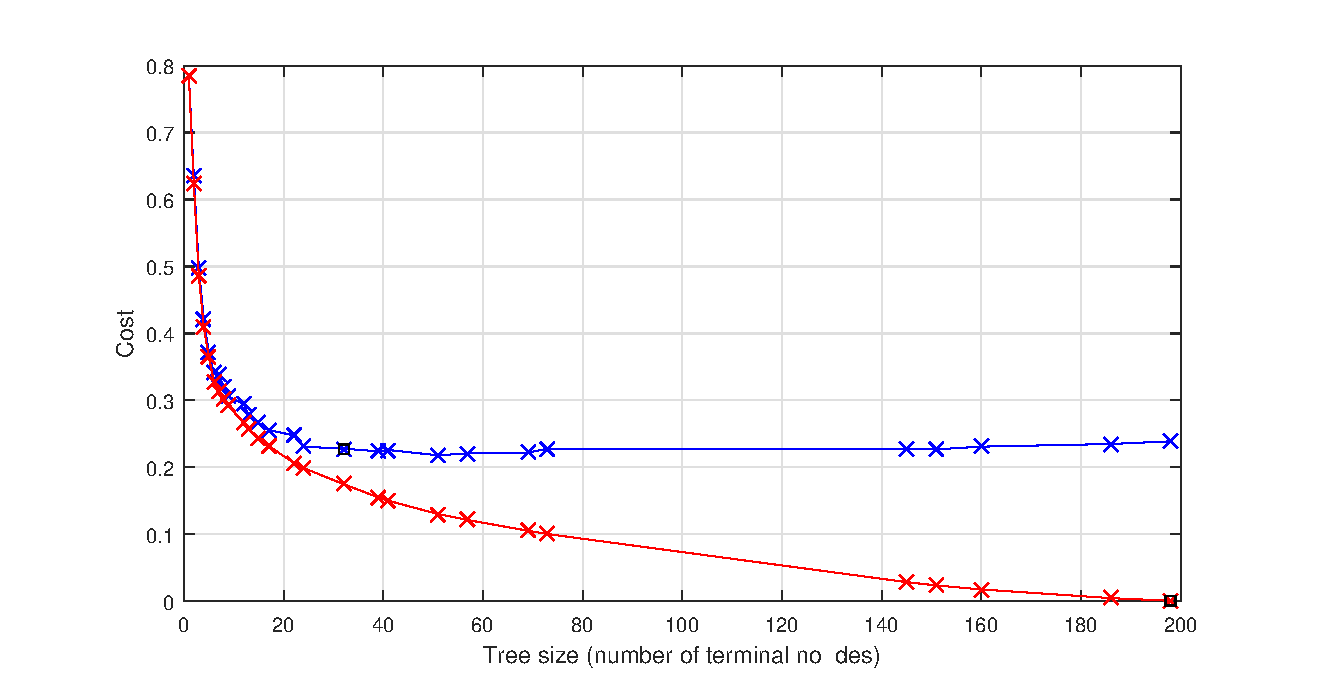
\includegraphics[scale=.7]{pruning_clean_data.eps}
%}
%\subcaptionbox{Pruning Example with noisy data}{
    %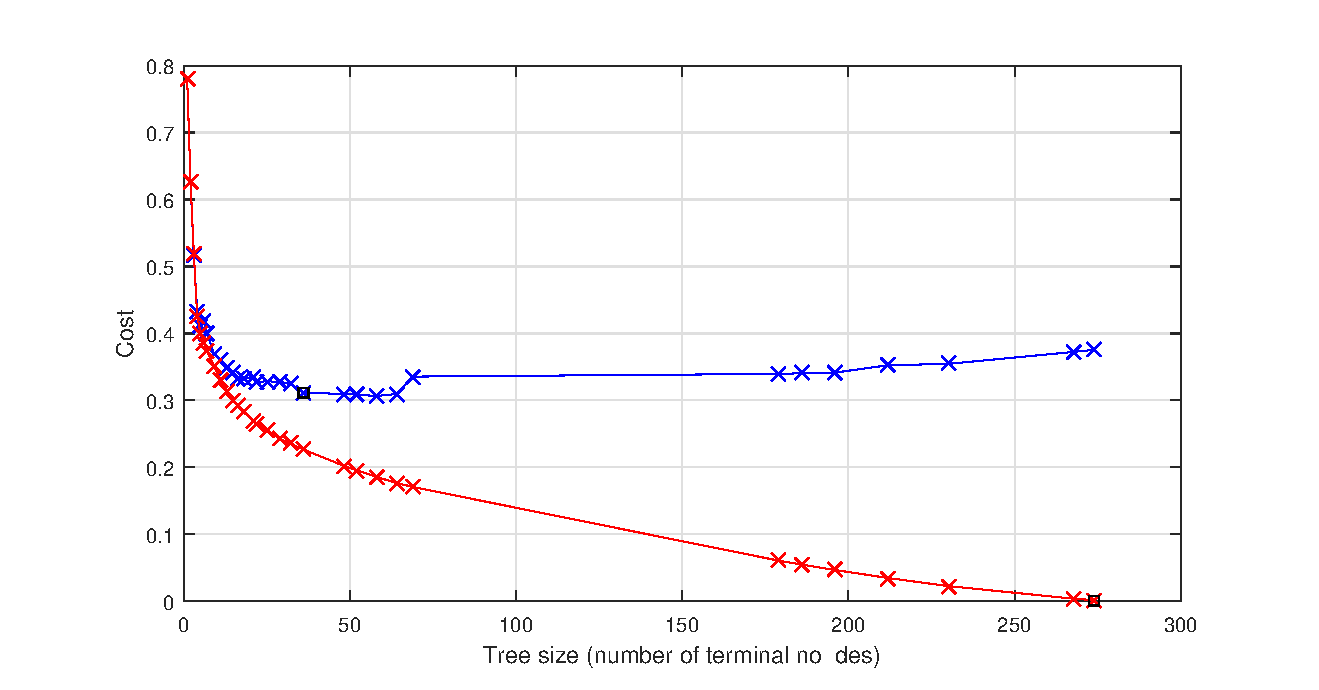
\includegraphics[scale=.7]{pruning_noisy_data.eps}
%}
%\caption{Plots produced by \emph{pruning\_example}}
%\label{fig:pruning}
%\end{figure}
%


%\bibliographystyle{plainnat}
%\bibliography{example}

\end{document}
